\chapter{Implementación}
     En este capítulo se explican los detalles de la implementación de las partes FrontEnd y BackEnd de nuestro proyecto, tanto de la generación del proyecto inicial como de la infraestructura del mismo.
    
    
    \section{FrontEnd}
    En esta sección se va a hablar del proyecto Angular el cual compone la parte FrontEnd de nuestra aplicación. Este framework nos ofrece un desarrollo más rápido con respecto a otros frameworks, ya que se estructura en diferentes componentes web y genera una página web dinámicamente.
    \subsection{Generación Proyecto Angular}
    Para la generación de un proyecto base en Angular se utilizó \textit{Angular Cli}, un herramienta de línea de comandos que facilita la creación y gestión de proyectos Angular y de sus diferentes componentes.
    \newline
    
    \textit{Angular Cli}, al tratarse de  una herramienta NodeJS, requiere tenerlo instalado en nuestro sistema operativo. Para ello la primera tarea a realizar es instalar NodeJS a través de su página oficial\cite{nodejs}, escogiendo la versión que soporte nuestro sistema operativo.
 
    A continuación, a través del terminal que nos proporciona la herramienta de desarrollo \textit{Visual Studio Code}, ejecutamos el comando \texttt{npm install -g @angular/cli@latest}, el cual nos instala \textit{Angular Cli} en la última versión disponible.
    
    \begin{figure}[h]
    \centering
     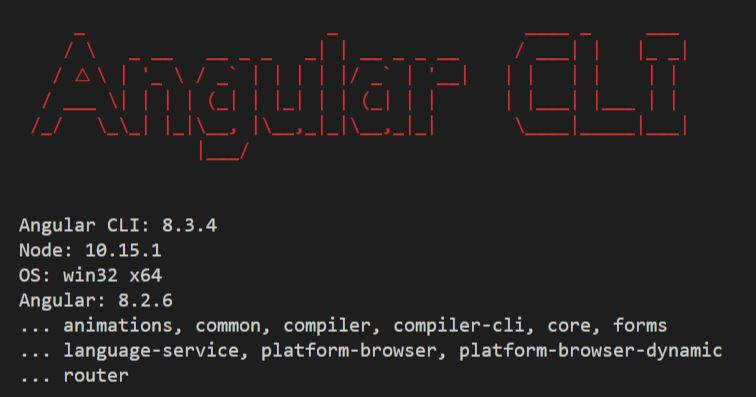
\includegraphics[width=0.65\textwidth]{images/angularversion}
    \caption{Versión Angular Cli}
    \end{figure}
    
    \FloatBarrier
    
    Una vez instalada la herramienta de comandos \textit{Angular Cli}, procedemos a crear nuestro proyecto base Angular ejecutando el comando \texttt{ng new estudio-medico-tfg2019}, generando un proyecto completo Angular junto con toda su estructura de carpetas.
    
    
    
    \subsection{Arquitectura de la aplicación Angular}
    
    \subsection{Inicialización del proyecto}
        \subsubsection{\underline{Local}}
        \subsubsection{\underline{Remoto}}
    
    
    \section{BackEnd}
    
     En esta sección se va a hablar del proyecto Java Spring Boot el cual compone la parte BackEnd de nuestra aplicación. La aplicación es una API-REST, la cual será consumida por el FrontEnd mediente llamadas en protocolo HTTP. 
     
     
    \subsection{Generación Proyecto Java Spring Boot}
    Para la generación del proyecto inicial se utilizó Spring Initializr\cite{springinitializr}, a través de su página web. Escogimos gestionar las dependencias del proyecto con Maven dado el alto grado de familiaridad que poseemos con esta tecnología. A continuación se escogió el lenguaje Java para implementar la aplicación debido a sus características intrínsecas(polimorfismo y herencia). Para finalizar se añadieron los paquetes de Web y JPA, necesarios para gestionar las conexiones externas y para la capa de persistencia.
    
    \begin{figure}[h]
    \centering
     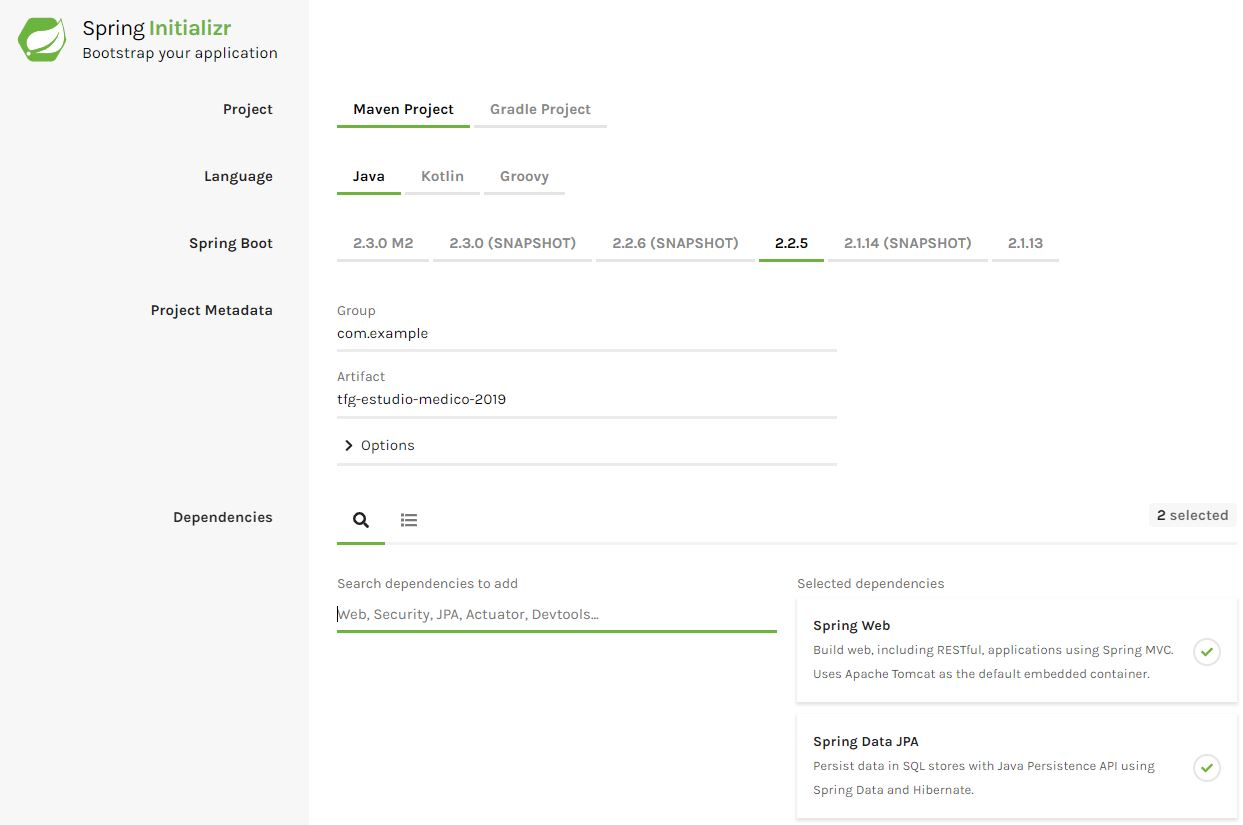
\includegraphics[width=1\textwidth]{images/springstarter}
    \caption{Proyecto inicial Spring Boot}
    \end{figure}
    
    Una vez generado el proyecto Sprinig Boot, hubo de importarse el mismo en el entorno de desarrollo Eclipse.
    
    
    \subsection{Arquitectura de la aplicación Java SPring Boot}
    La aplicación Spring Boot desarrollada se divide principalmente en cuatro carpetas o bloques: java, recursos, test  y el archivo pom.xml. Dichos bloques se explicarán con detalles en las secciones a continuación.

        \subsubsection{\underline{Bloque java}}
        \subsubsection{\underline{Bloque test}}
        \subsubsection{\underline{Bloque resources}}
        \subsubsection{\underline{Bloque pom.xml}}
        
        
    \subsection{Inicialización del proyecto}
        \subsubsection{\underline{Local}}
        \subsubsection{\underline{Remoto}}
    